\chapter{Theory}

This chapter serves to introduce relevant theory on which the thesis rests. 

We will briefly review EEG, and some of the machine learning techniques used.

\section{Electroencephalography (EEG)}\label{eeg-theory}

    Electroencephalography is a method used to measure the activity of neurons in the brain by recording the electrical activity on the scalp.

    As a non-invasive method it is widely used in medicine to diagnose and study a wide range of conditions, including epilepsy and sleep disorders.

    In research it has also found use in studying ``Event Related Potentials'', or ERPs, which are stereotyped responses to a stimulus. Common ERPs can be seen in Table~\ref{table:erps}.

    \add[inline]{Plot of aggregated ERP trials, to highlight an ERP pattern (found in eeg-notebooks examples)}

    \begin{table}
        \begin{tabular}{ll}
            \toprule
            ERP & Description
            \\
            \midrule
            N170 & Elicited by processing of faces, familiar objects or words.
            \\
            N400 & Elicited by words and other stimuli.
            \\
            P600 & Elicited by hearing or reading grammatical errors and other syntactic anomalies.
            \\
            \bottomrule
        \end{tabular}
        \caption{Common ERPs}\label{table:erps}
    \end{table}

    Electrodes can be placed at different locations on the scalp, targeting different regions of the brain. The system used to position the electrodes is called the 10–20 system (seen in Figure~\ref{fig:1020}), and is the standard way to label electrode placements. The \emph{10} and \emph{20} come from the fact that distances between adjacent electrodes are either 10\% or 20\% of the total front–back or right–left distance of the scalp.

    For configurations with high-density or non-standard electrode placement there is also the \emph{Modified Combinatorial Nomenclature} (MCN) version with more electrode locations, where the electrodes are divided by 10\% increments instead of the usual 20\% (seen in Figure~\ref{fig:1020-extended}).

    \begin{figure}
        \begin{center}
            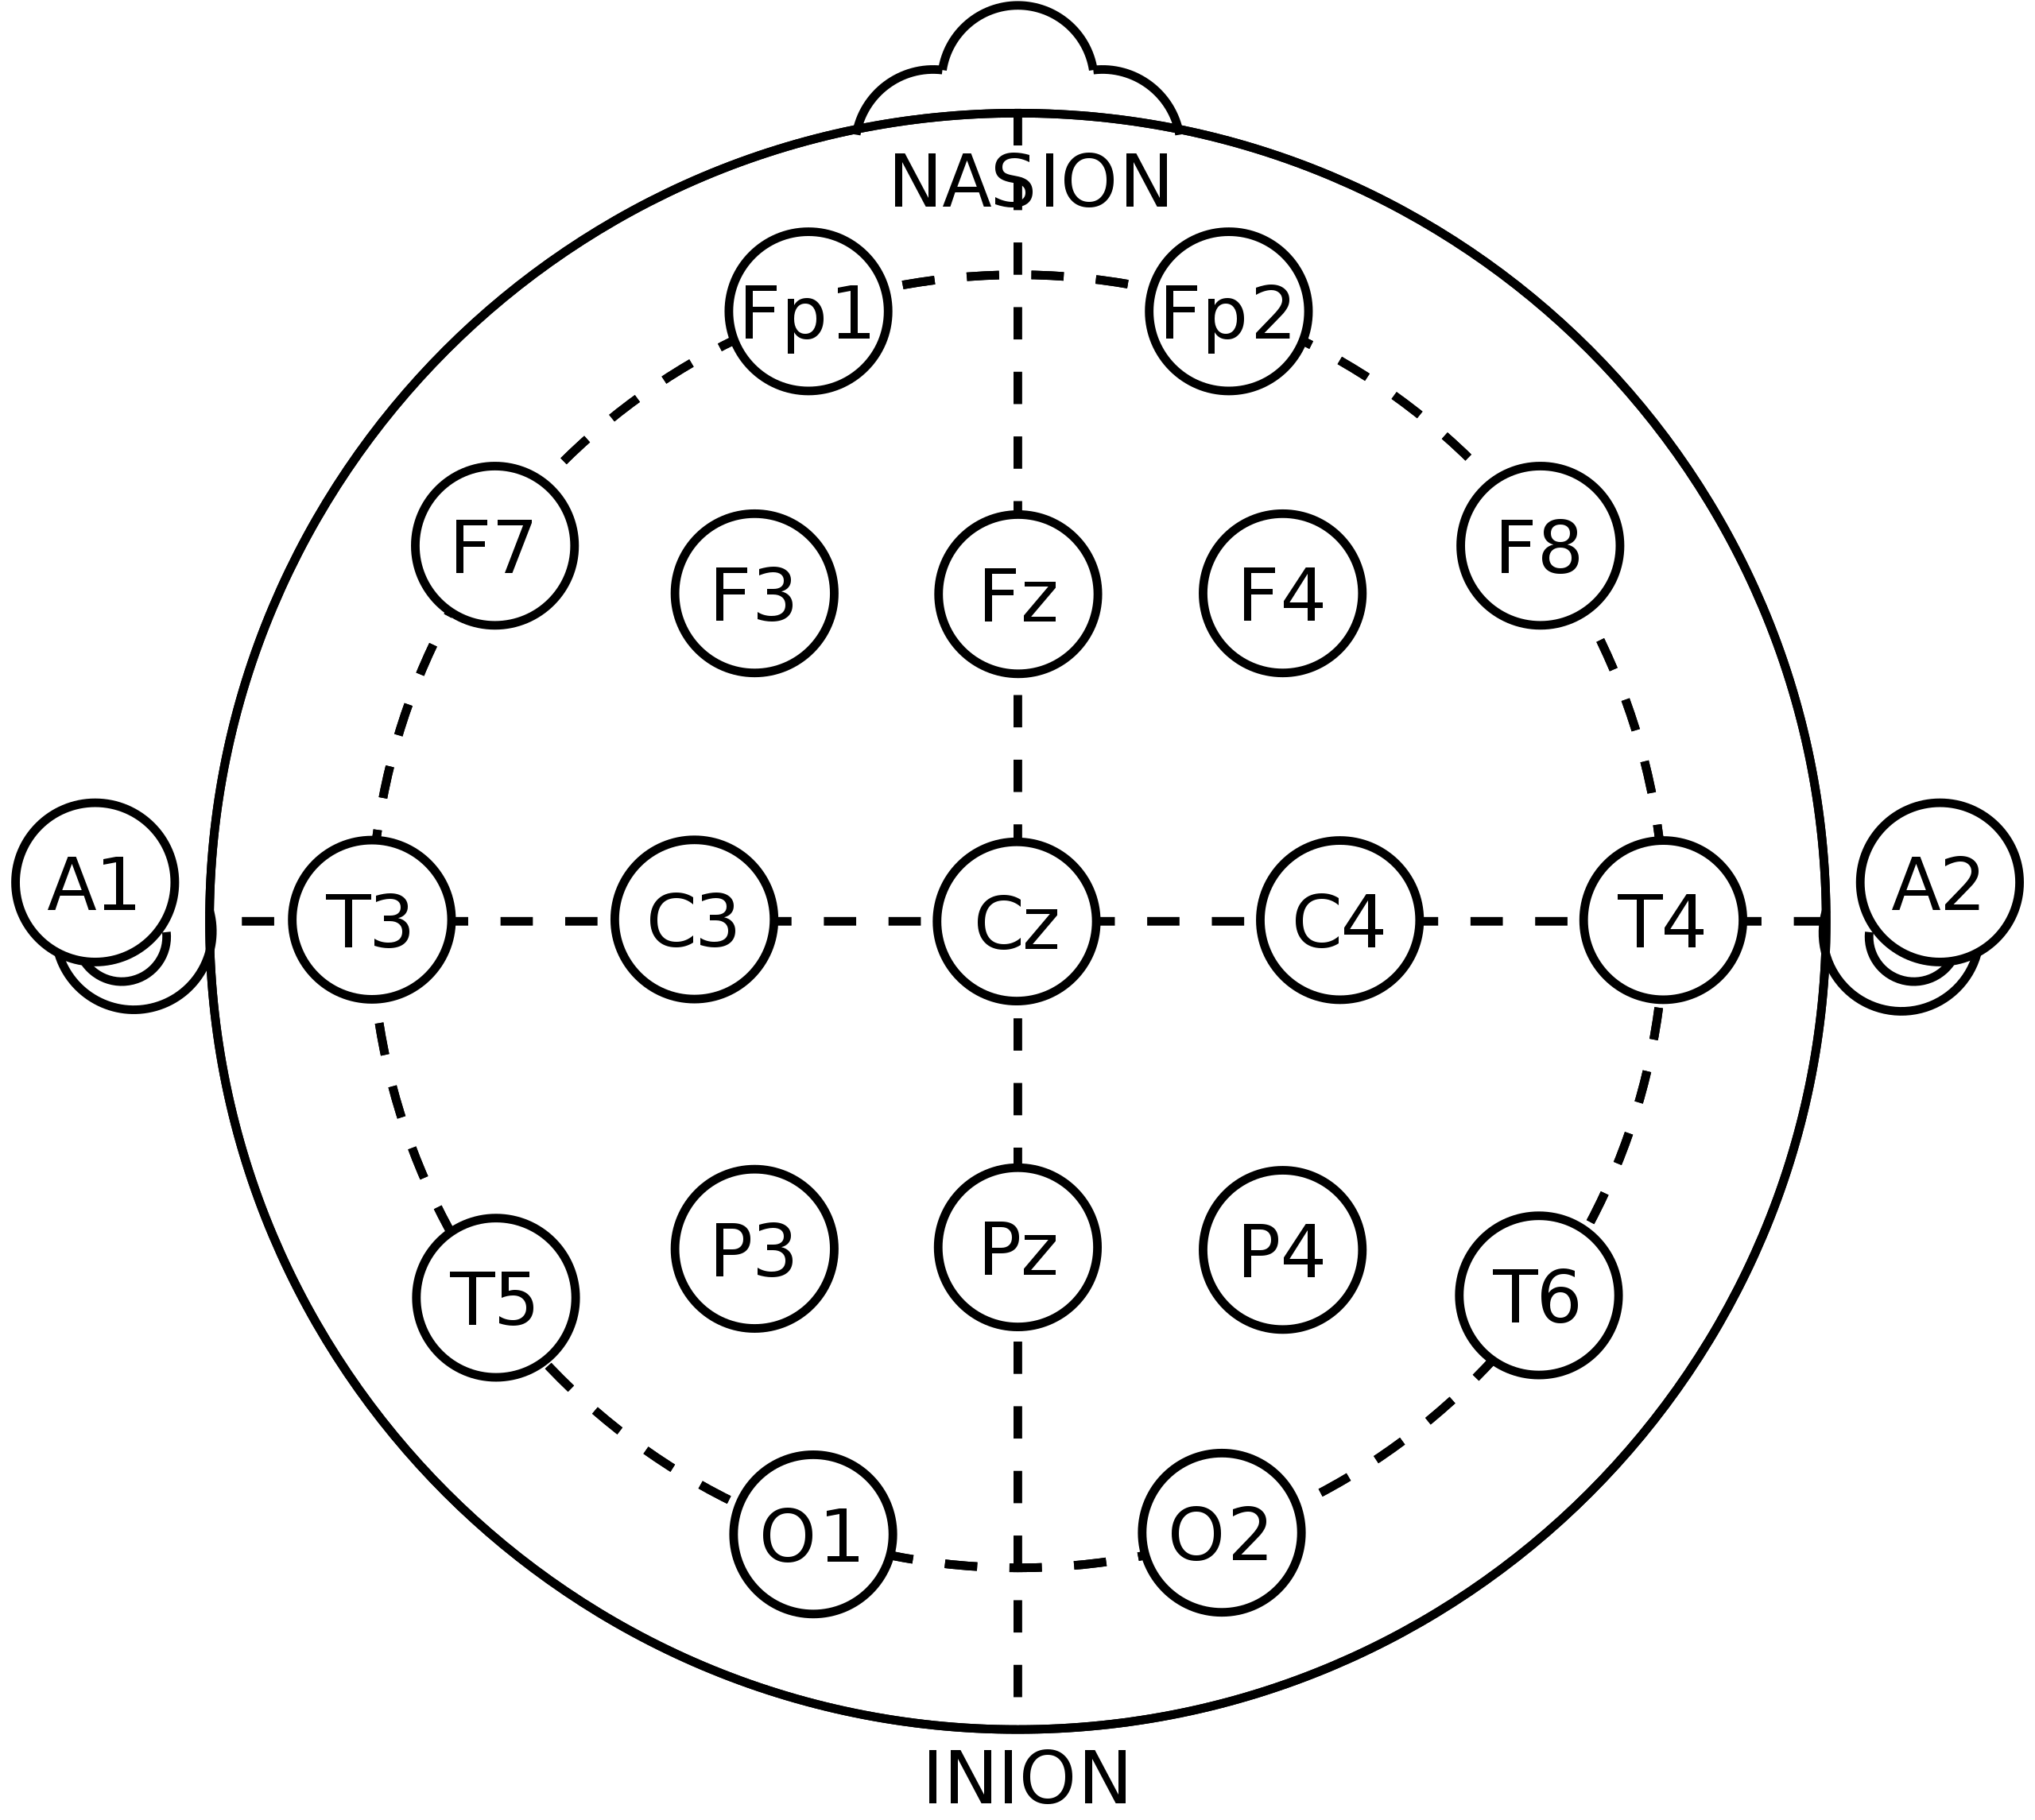
\includegraphics[width=10cm]{img/1020system.png}
        \end{center}
        \caption{The 10–20 system.}\label{fig:1020}
    \end{figure}

    \begin{landscape}
        \begin{figure}
            \begin{center}
                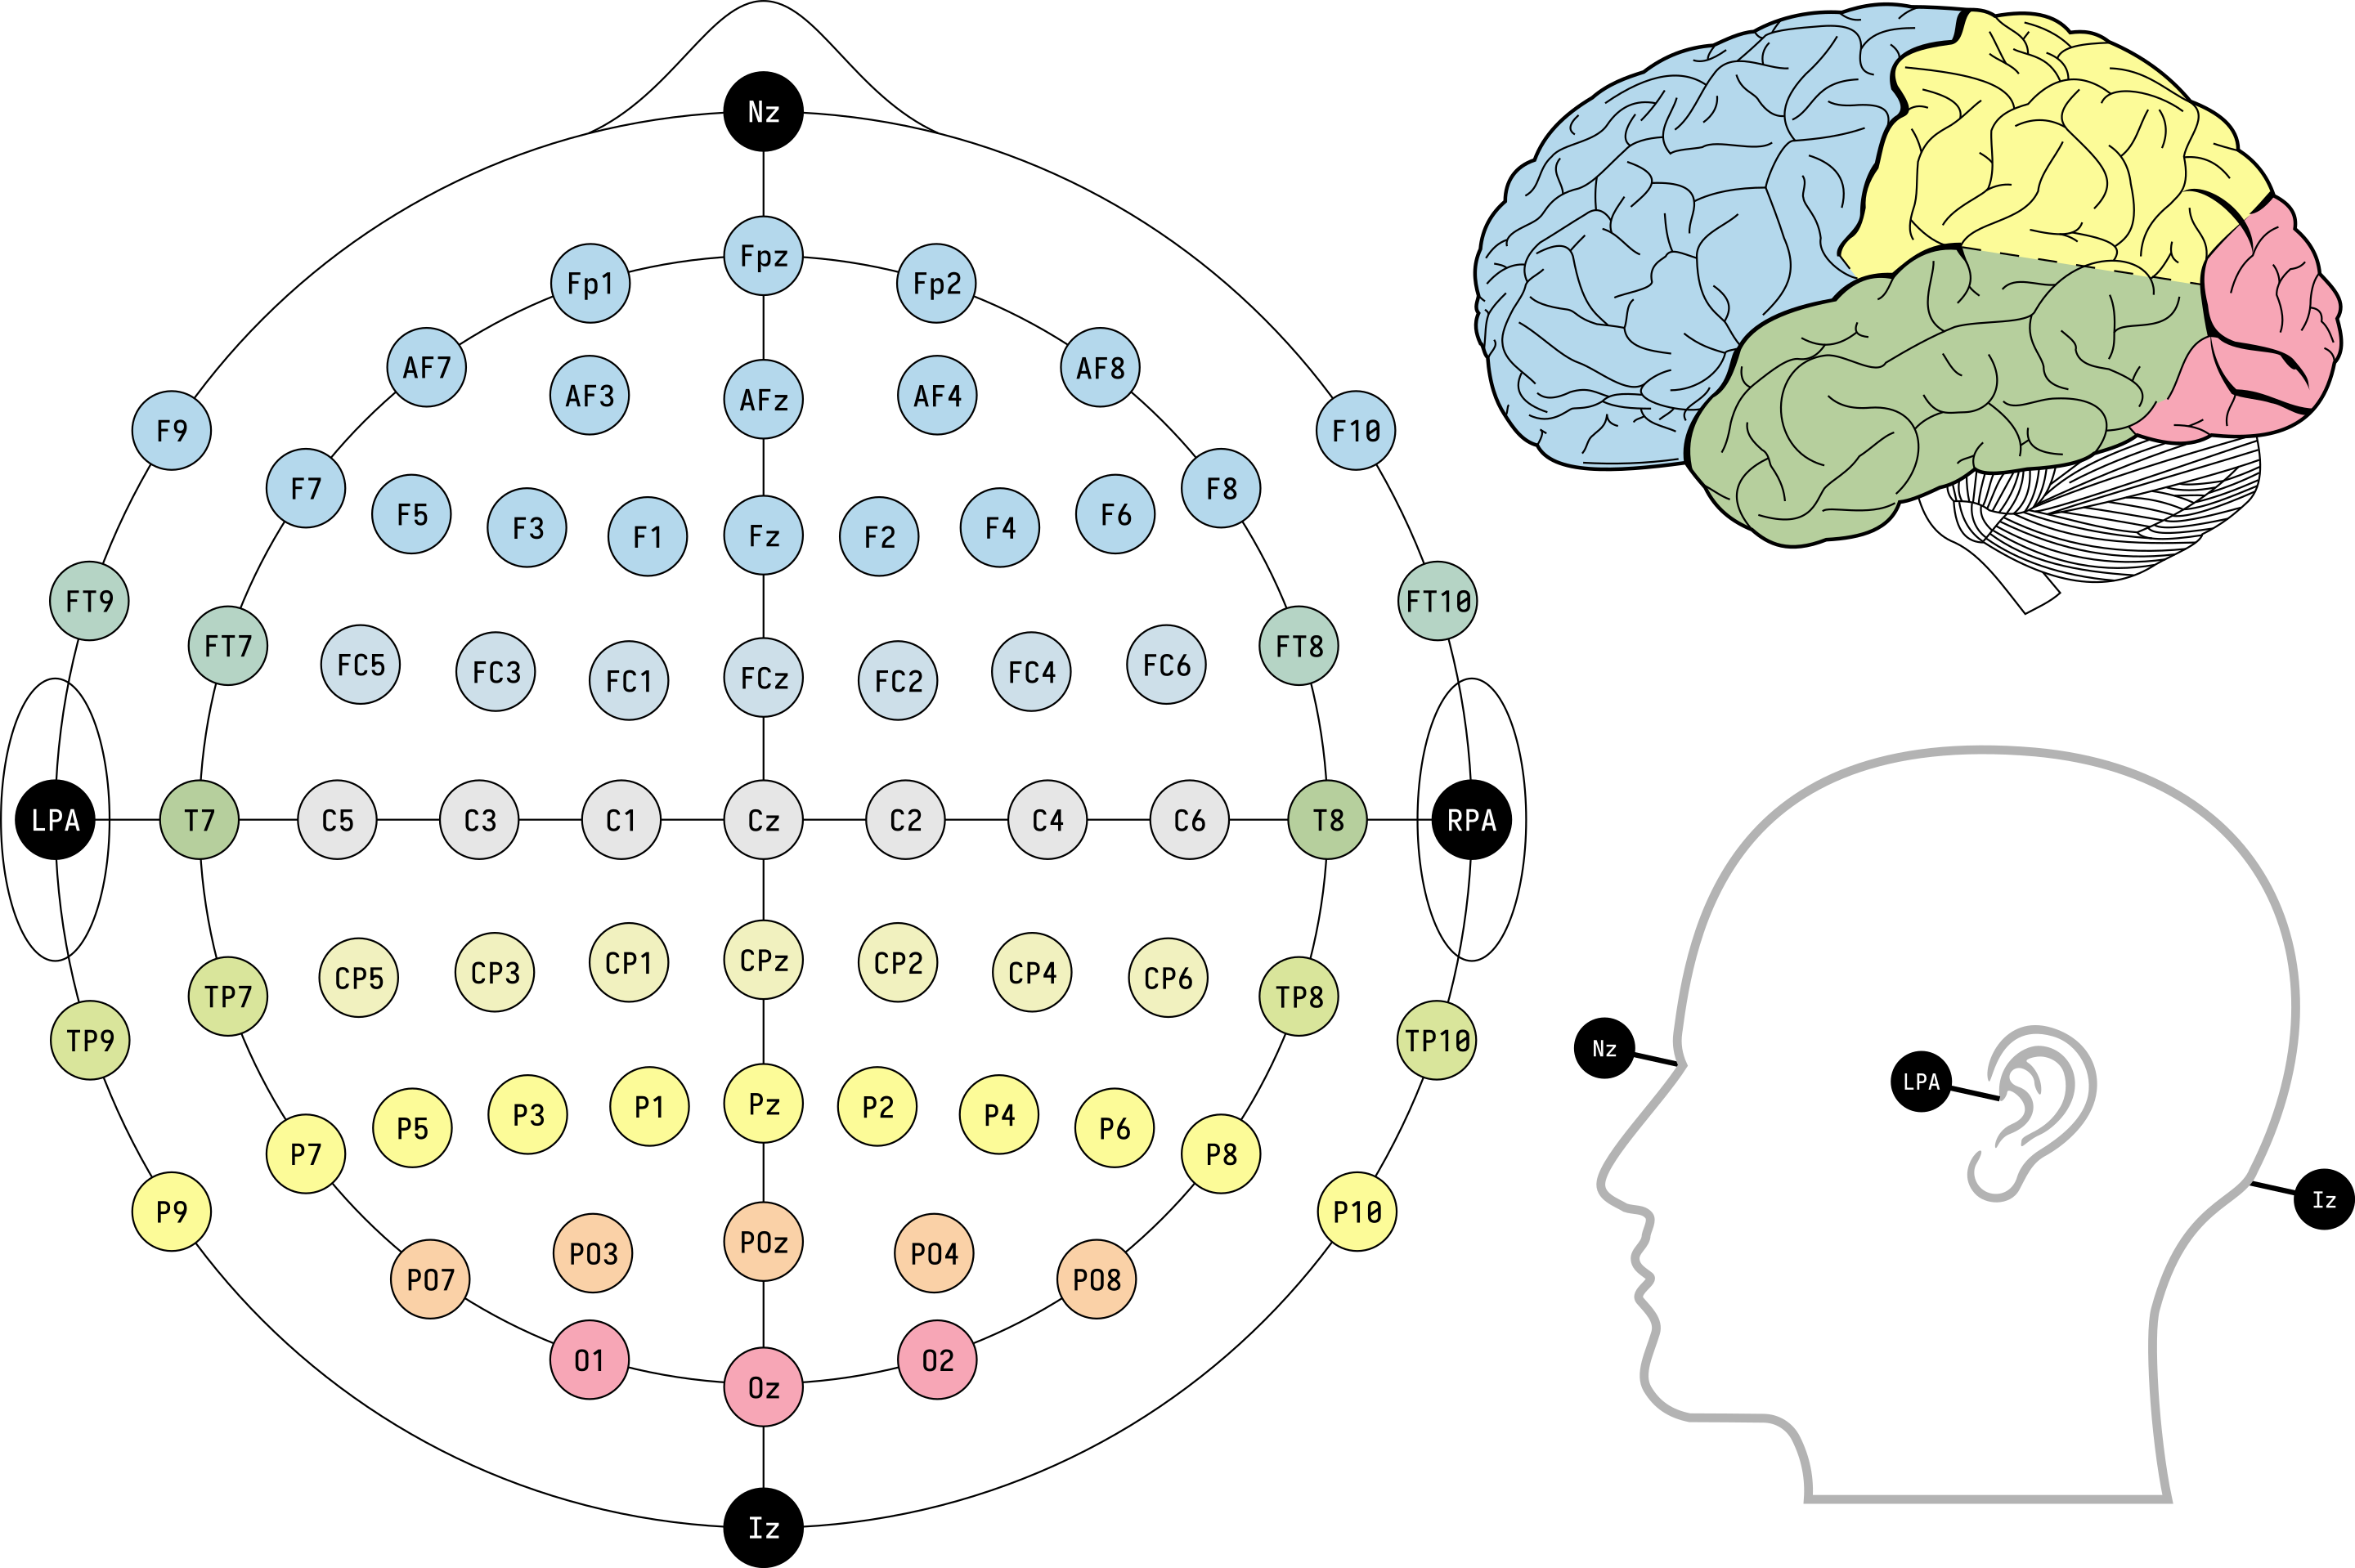
\includegraphics[width=20cm]{img/1020system-extended-with-extra-info.png}
            \end{center}
            \caption{The extended 10–20 system, following the Modified Combinatorial Nomenclature (MCN).}\label{fig:1020-extended}
        \end{figure}
    \end{landscape}

    As measurements are taken on the scalp, neural activity of surface-level neurons (such as the cerebral cortex) can be expected to dominate the signal, which makes it difficult to use when studying systems deeper in the brain (such as the hippocampus). As an example of this, eye blinks are easily identifieable in the signal when electrodes are placed on the frontal cortex (seen in Figure~\ref{fig:muselsl-signal}).

    \add[inline]{Plots of PSD, PCA, etc}
    \add[inline]{Mention need for bandpass filtering to get rid of powerline noise}

    \add[inline]{Discuss some of the review articles on EEG/BCI/ML}

    \begin{landscape}
        \begin{figure}
            \begin{center}
                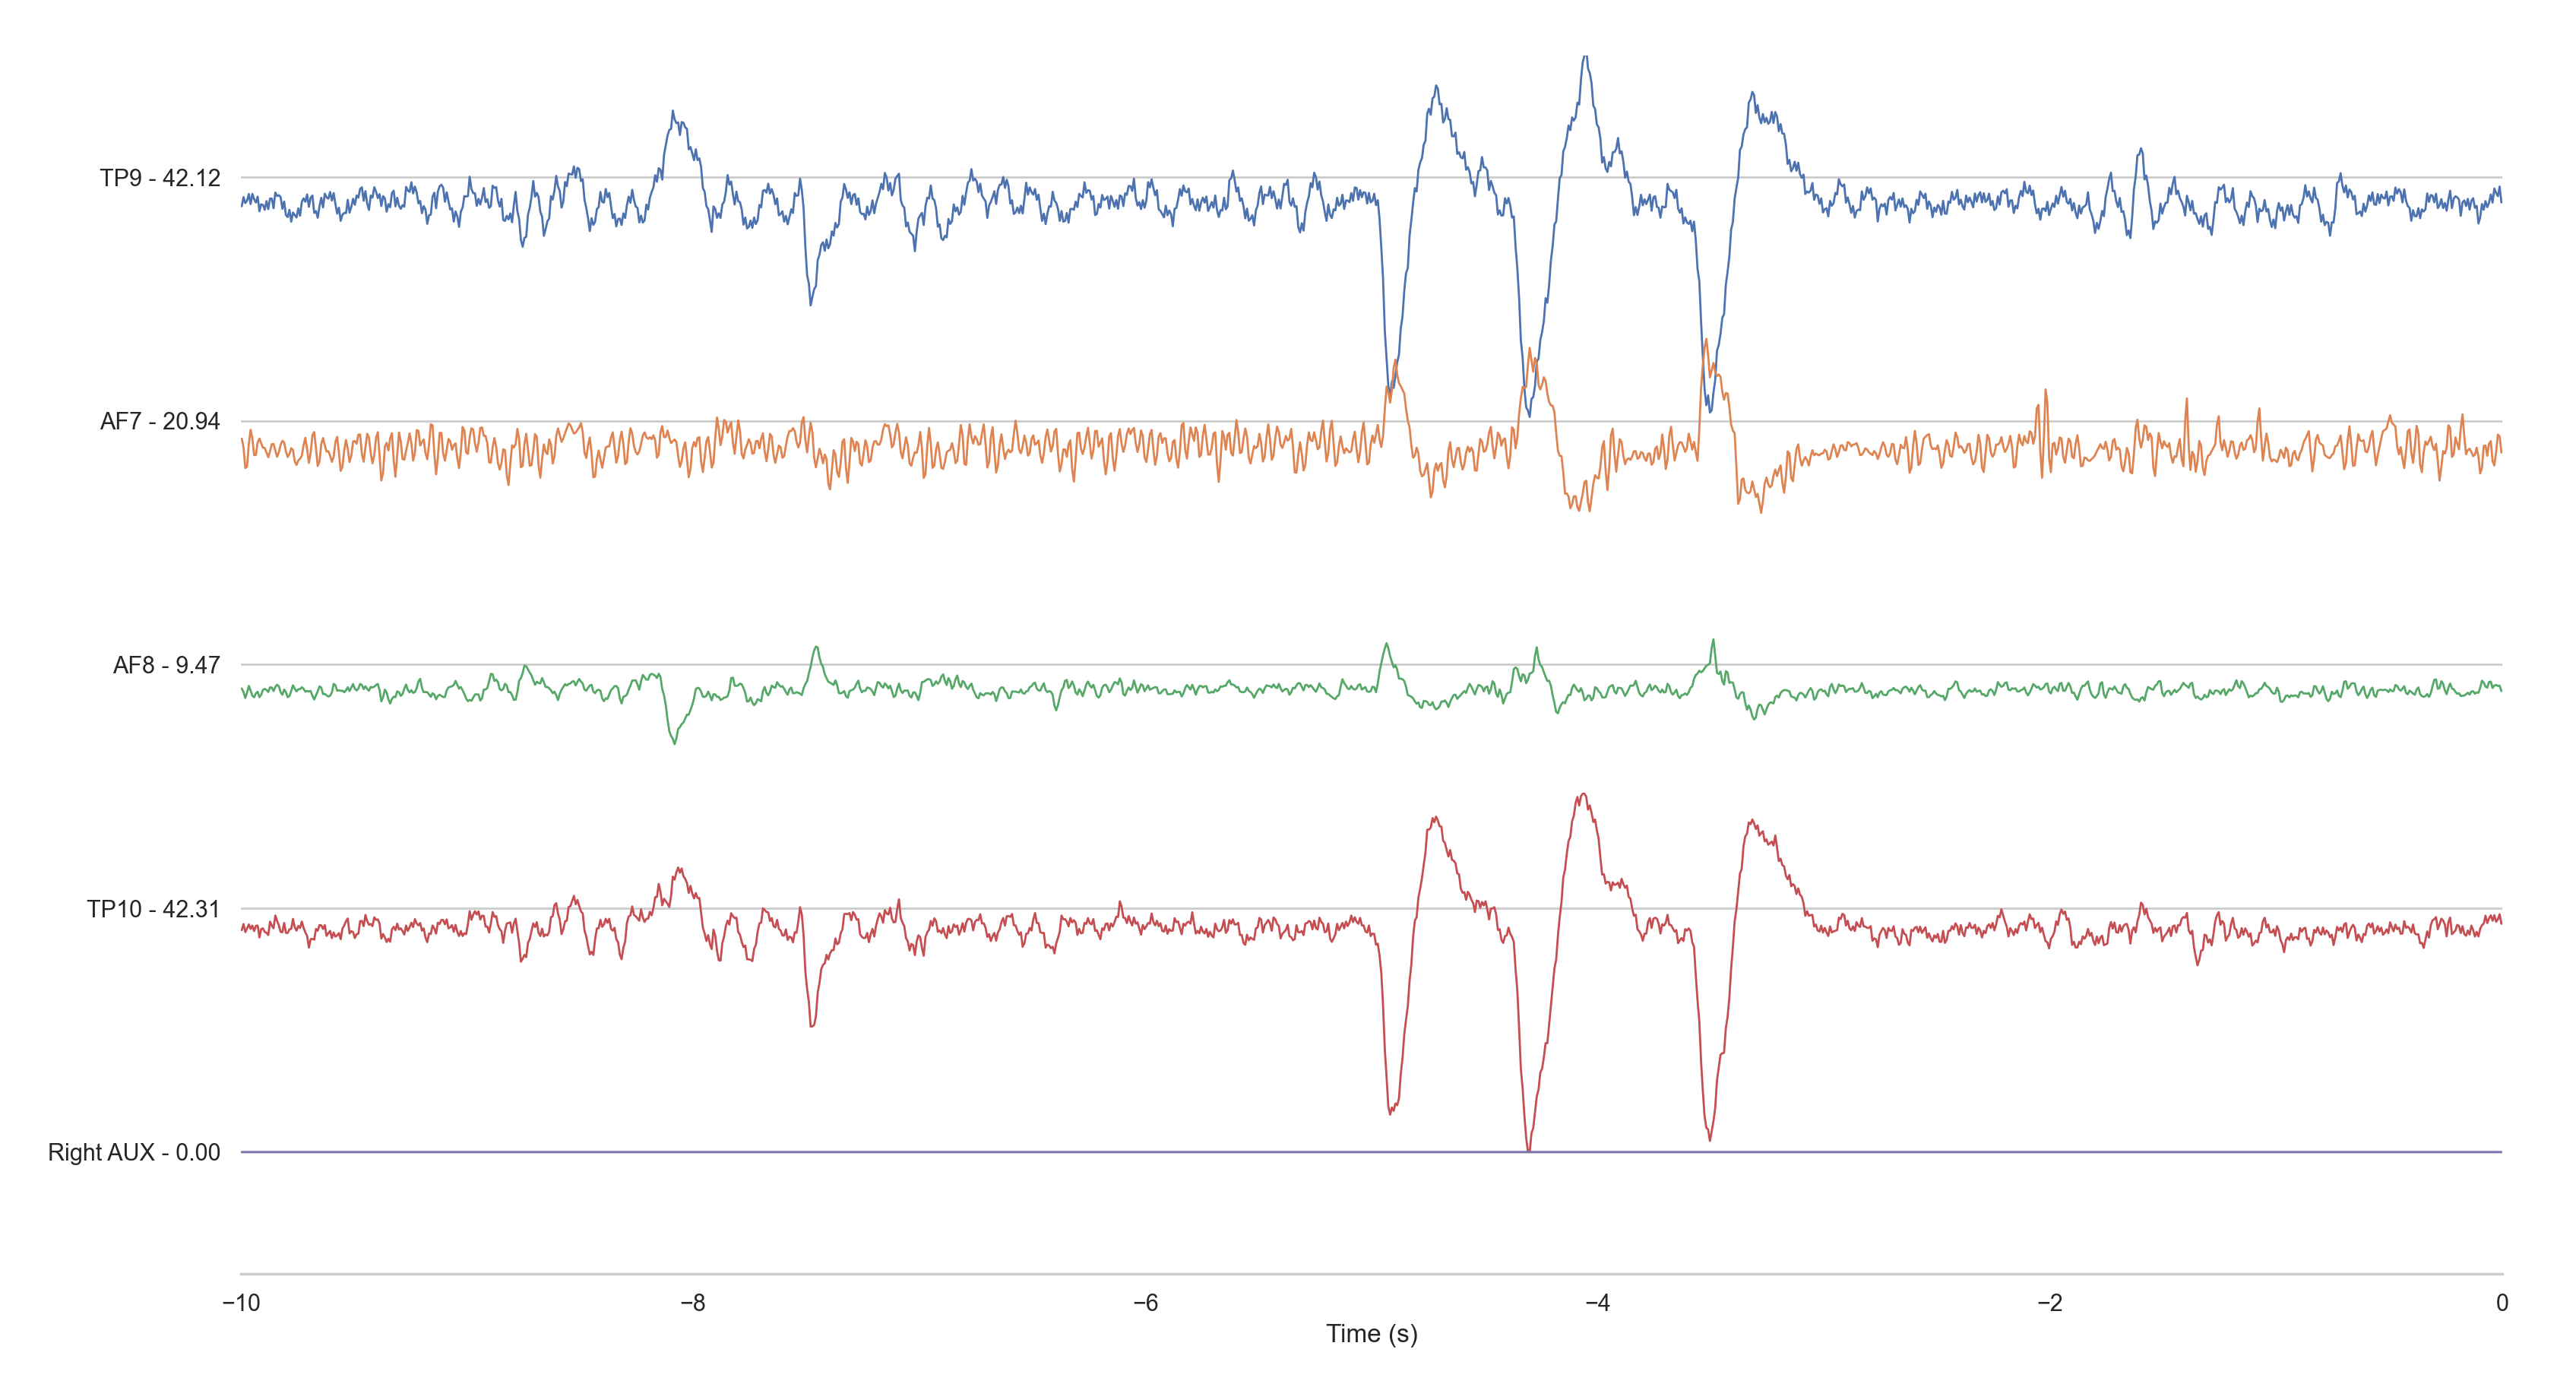
\includegraphics[trim=60 50 50 60,clip,width=24cm]{img/muselsl-signal.png}
            \end{center}
            \caption{EEG signal viewed with muse-lsl. There are 3 eye blinks identifiable around $\SI{-4}{\second}$.\\ The signal has been bandpass filtered to eliminate noise.}\label{fig:muselsl-signal}
        \end{figure}
    \end{landscape}

\section{Machine Learning}

    Machine learning on EEG data utilizes several domain-specific methods (which?) often similar to other methods seen applied to general time-series data.

    Among these we find methods like bandpass filtering, windowing, spectral density estimation, and the computation of covariance matrices to estimate interdependencies between channels.

    Methods used in analysis and classification of EEG data include Linear Discriminant Analysis (LDA), Common Spatial Pattern (CSP)~\cite{barachant_common_2010} filters.

    With the use of these methods, we can compute features to use when training our classifiers.

    The underlying ML algorithms themselves are often off-the-shelf logistic regression, with some domain adaptations found in more complex models like neural networks.

    \add[inline]{Formulas}

    \subsection{Riemannian geometry}\label{section:riemannian-theory}

        \add[inline]{Explanation of Riemannian geometry, from \href{https://colab.research.google.com/drive/1y9tq7-lJwusxtVgpB38y-p1pYw7hg0iu}{this tutorial we're working on}, perhaps it should go in the Background/Theory section though?}

        The Riemannian distance measure for two symmetric positive definite matrices (such as a covariance matrix) is:~\cite{grafarend_metric_2003}

        \[ d(A, B) = \sqrt{\sum_{i=1}^{n} \ln^2 \lambda_i (A, B) } \]

    \subsection{Neural networks}

        Many state-of-the-art models in the field of EEG are deep-learning based models, usually employing convolutional neural networks (CNNs).
